\documentclass{beamer}
%\hypersetup{bookmarksopen=true,bookmarksopenlevel=4}
\setcounter{tocdepth}{2}

\usepackage[utf8]{inputenc}
\usepackage[T1]{fontenc}
\usepackage{mathtools}
\usepackage{hyperref}
\usepackage{multicol}
\usepackage{tcolorbox}
\usetheme{metropolis}  

\title{Optimal Control and Optimization in Robotics}

\author{Mengda Li}
\institute{ENS Paris-Saclay}

\begin{document}

\begin{frame}
\titlepage
\end{frame}



\begin{frame}{Introduction}
%\section*{Introduction}
My internship is co-supervised by Justin Carpentier (Willow, Inria Paris) and Nicolas Mansard (Gepetto, LAAS/CNRS) in the Willow research group at INRIA Paris in France. 


\begin{columns}
\column{0.5\textwidth}
\begin{figure}
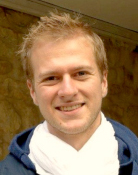
\includegraphics[scale=0.35]{images/Justin_Carpentier.jpg}
\caption{Justin Carpentier}
\end{figure}
\column{0.5\textwidth}
\begin{figure}
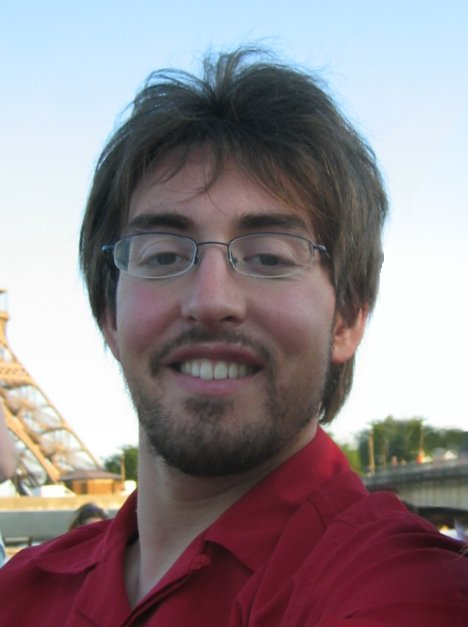
\includegraphics[scale=0.1]{images/Nicolas_Mansard.jpg}
\caption{Nicolas Mansard}
\end{figure}
\end{columns}

\end{frame}

\begin{frame}{Hosting institution}

\begin{figure}

\includegraphics[scale=0.35]{images/Inr_logo_fr_rouge.png}
%\caption{}
\end{figure}
L'\textbf{Institut national de recherche en informatique et en automatique (Inria)} est un établissement public à caractère scientifique et technologique français spécialisé en mathématiques et informatique, placé sous la double tutelle du ministère de l'Enseignement supérieur, de la Recherche et de l'Innovation et du ministère de l'Économie et des Finances créé le 3 janvier 1967 dans le cadre du « plan calcul ».





\end{frame}


\begin{frame}{Research teams}

\begin{figure}

\includegraphics[scale=0.3]{images/WILLOW_Research.png}
%\caption{}
\end{figure}

\textbf{WILLOW} is based in the Laboratoire d'Informatique de l'École Normale Superiéure (CNRS/ENS/INRIA UMR 8548) and is a joint research team between INRIA Rocquencourt, École Normale Supérieure de Paris and Centre National de la Recherche Scientifique. 

Their research is concerned with representational issues in visual object recognition and scene understanding. 



\end{frame}

%\begin{frame}{Research teams II}
%
%
%Gepetto, LAAS/CNRS:..
%\end{frame}

\begin{frame}{Motivations and Problems in a general context}

I want my robot to move one thing somewhere and pass some point at some moment with a lowest cost.

\bigskip

\textbf{Optimization}: lowest cost

\textbf{Control}: from some point to another point

and \emph{Constraints}
\end{frame}


\begin{frame}{Outline}
%\begin{multicols}{2}
\tableofcontents
%\end{multicols}
\end{frame}

\section{Optimal Control Problem}

  \begin{frame}{Optimal Control	Problem}
    \subsubsection{Goal 1: Controllability}

Goal 1: Controllability
	\begin{equation}
	\begin{aligned}
	& {\text{find}}
	& & u \\
	& \text{subject to}
	& & x(0) = x_0, \; x(T) = p, \\
	&&& \dot{x} (t) = f(x(t), u(t)).
	\end{aligned}
	\end{equation}
	
	\subsubsection{Goal 2: Optimal Control}

Goal 2: Optimal Control	 
	
	\begin{equation}
	\begin{aligned}
	& \underset{u}{\text{minimize}}
	& & \int_0^T l(x(t),u(t)) dt \\
	& \text{subject to}
	& & x(0) = x_0, \; x(T) = p, \\
	&&& \dot{x} (t) = f(x(t), u(t)).
	\end{aligned}
	\end{equation}
	
  \end{frame}
  
  \begin{frame}{Transformation of the problem}
  \subsection{Transformation of the problem}
 \subsubsection{Adding penalty}
Adding penalty to the terminal lost:
\begin{equation}
\begin{aligned}
& \underset{u}{\text{minimize}}
& & \int_{[0,T[} l(x(t),u(t)) dt + l_T(x(T)) \\
& \text{subject to}
& & x(0) = x_0,  \\
&&& \dot{x} (t) = f(x(t), u(t)).
\end{aligned}
\end{equation}

\subsubsection{Discretization}
Discretization of functions and variables:
\begin{equation}
\label{eq}
\begin{aligned}
&\underset{x \in \ell_{N+1}^\infty, u \in \ell_{N}^\infty}{\text{minimize}}          &J(x, u) &=\sum_{i = 0}^{N-1} L(x_i, u_i) + L_T(x_N) \\
&\text{subject to}       &x(0)      &= x_0,  \\ %or \epsilon_{0} 
&							      &x_{i+1}  &= F(x_i, u_i) \ \forall i \in [0 .. N-1]
\end{aligned}
\end{equation}
  \end{frame}
  
\addtocontents{toc}{\newpage}
\section{Differential Dynamic Programming}
\subsection{Dynamic Programming}
\begin{frame}{Dynamic Programming}
Optimize one by one:
\begin{equation}
\begin{split}
\min_{U} J(U) &= \min_{u_0} \min_{u_1} ... \min_{u_{N-1}} J(U)
\end{split}
\end{equation}
Definitions of Value Function and Q-functions:
\begin{equation}
\begin{split}
\label{vl}
V_i(x_i ) &= \min_{u_i}L(x_i,u_i) + V_{i+1}(x_{i+1}) \\
		V_N(x_N) &= L_T(x_N)
\end{split}
\end{equation}

\begin{equation}
\begin{split}
Q_i(x_i,u_i) &= L(x_i,u_i) + V_{i+1}(x_{i+1}) \\
				&= L(x_i,u_i) + V_{i+1}(f(x_i,u_i)) \\
				&= L(x_i,u_i) + \min_{u_{i+1}} Q_{i+1}(f(x_i,u_i), u_{i+1}),\ i \le N-2
\end{split}
\end{equation}

\begin{equation}
V_i(x_i) = \min_{u_i} Q_i(x_i, u_i) 
\end{equation}
\end{frame}

\subsection{Linear Quadratic Regulator (LQR)}

\begin{frame}{Linear Quadratic Regulator (LQR)}
The LQR is an algorithm that solves the problem \ref{eq} \emph{ in one iteration}
in case $L, L_T$ are \textbf{quadratic} and $F$ is \textbf{linear} (or quadratic). 

\medskip

Two phases in the algorithm: 
\begin{itemize}
\item \textbf{Backward and Forward pass}: 

Compute $V_x, V_{xx}$ and $Q_u, Q_{uu}, Q_{ux}$ alternately

\item \textbf{Roll-out}: 

Compute $\delta_u^*$ by $V_x, V_{xx}$ and $Q_u, Q_{uu}, Q_{ux}$

\end{itemize}

%\textbf{Backward and Forward pass}: 
%\begin{center}
%Compute $V_x, V_{xx}$ and $Q_u, Q_{uu}, Q_{ux}$ alternately
%\end{center} 

\end{frame}

\subsubsection{Backward and Forward pass}

\begin{frame}{Backward and Forward pass}

\textbf{Backward} pass: from the partial derivatives of $V_{i+1}$ back to the partial derivatives of $Q_i$
\begin{equation}
\label{QfromV}
\begin{split}
Q_u & = L_u + \underline{V'_x}   \ F_u \quad \footnotemark \\
Q_{uu} &= L_{uu} + \underline{V'_x} \cdot F_{uu} + F_u^T \underline{V'_{xx}} F_u \\
Q_{ux} &= L_{ux} + \underline{V'_x} \cdot F_{ux} + F_u^T \underline{V'_{xx}} F_x
\end{split}
\end{equation}

\footnotetext{"$Q, V'$" mean "$Q_i, V_{i+1}$".}

\textbf{Forward} pass: from the partial derivatives of $Q_i$ back to the partial derivatives of $V_i$
\begin{equation}
\label{VfromQ}
\begin{aligned}
V_x &= Q_x - Q_u Q_{uu}^{-1} Q_{ux} &=& Q_x + Q_u K \\
V_{xx} &= Q_{xx} - Q_{xu} Q_{uu}^{-1} Q_{ux} &=& Q_{xx} + Q_{xu} K
\end{aligned}
\end{equation}

\end{frame}


\begin{frame}{Roll-out}
\subsubsection{Roll-out}
Roll-\textbf{out}: determine the new trajectory $x, u$ by computing the best control change $\delta_u$.

\begin{equation}
\begin{split}
\delta_u^* (i) &:= \arg\min_{\delta_u(i)}Q_i(x_i + \delta_x(i), u_i + \delta_u(i) ) \\
\delta_u^* &=  - Q_{uu}^{-1} (Q_u + Q_{ux} \delta_x) \quad \forall i \in [0 .. N-1]
\end{split}
\end{equation} 
%The idea is that we suppose for all $i$, $u_{i+1} ... u_{N-1}$ are already optimal, then we optimize $u_i$.
\begin{equation}
\begin{split}
u^* &:= u + \delta_u^*, \\
x^*_0      &= x_0,  \\ %or \epsilon_{0} 
x_{i+1}^*     &= F(x_i^*, u_i^*) \quad \forall i \in [0 .. N-1]
\end{split}
\end{equation}

\end{frame}

\begin{frame}	{Sequential Quadratic Programming (SQP)}
What if the $F, L$ are not quadratic? Use the Sequential Quadratic Programming to solve general non-linear problems.

\begin{equation}
\begin{aligned}
&\underset{x}{\text{minimize}}       &f(x) &\\
&\text{subject to}       &c(x) &= 0
\end{aligned}
\end{equation}

\begin{equation}
A(x)^T = [\nabla c_1(x), \nabla c_2(x),..., \nabla c_m(x)]
\end{equation}
Goal: KKT necessary conditions
\begin{equation}
F(x, \lambda) = \begin{bmatrix}
\nabla f(x) - A(x)^T \lambda \\
c(x)
\end{bmatrix} = 0
\end{equation}
Resolve the quadraticalized problems sequentially to find an optimal step and update the trajectory with a roll-out policy (like line search). 
\color{gray} \quad Partie technique, voir la chapitre 18 de  \cite{NoceWrig06} and \cite{crocoddyl}
\end{frame}


\section{Augmented Lagrangian method}

\begin{frame}{Penalty method}
\subsection{Penalty method}
The \emph{Penalty method} transform a \emph{constrained optimization problem}:
\begin{equation}
\begin{aligned}	
&\underset{x}{\text{minimize}}                  &f(x) &  & \\
&\text{subject to}     & c_i(x)  &= 0,  & i \in \mathcal{E}
\end{aligned}
\end{equation}
to an \emph{optimization problem without constraint}:
\begin{equation}
\label{eq: penalty}
\begin{aligned}	
&\underset{x}{\text{minimize}}       &f(x) + \frac{\mu}{2} \sum_{i \in \mathcal{E}} c_i^2(x),&  &\mu >0
\end{aligned}
\end{equation}
$\mu$ is the penalty parameter. We solve sequentially the \ref{eq: penalty} with an increasing sequence\footnote{For example, $\mu_{k+1} = 2 \mu_k$ if some residual tolerance is satisfied.} of $\mu_k$ until the final convergence test \footnote{For example, the residual $\|c(x)\| < 10^{-8}$}is satisfied.

\end{frame}

\subsection{Augmented Lagrangian}
\begin{frame}{Augmented Lagrangian}
\emph{Augmented Lagrangian function} is modified version of the \emph{penalty function}:
\begin{equation}
\label{eq:LA}
\mathcal{L}^A (x):= f(x) + \sum_{i \in \mathcal{E}} \lambda_i c_i(x) +\frac{\mu}{2} \sum_{i \in \mathcal{E}} c_i^2(x)
\end{equation}
The $\lambda$ is the dual variable called \emph{Lagrangian multiplier} who has the same dimension as the constraints.

While solving sequentially the \ref{eq:LA},
at each iteration,
\begin{itemize}
 \item if the tolerance is satisfied,  update $\lambda^{k+1} := \lambda^{k} + \mu^k c(x_k)$
 \item else, increase the penalty $\mu$
 \item Stopping criteria: KKT necessary optimality conditions 
\end{itemize}

If the algorithm finally finds a numerical optimum, the final $\lambda$ would also be the dual optimum numerically.
\end{frame}


\begin{frame}{Central problem in the internship}
\begin{equation}
\label{eq:OCP equality constraints}
\begin{aligned}
&\underset{x \in \mathbb{X}^{T+1}, u \in \mathbb{U}^T}{\text{minimize}}          &J(x, u) &=\sum_{i = 0}^{T-1} L_i(x_i, u_i) + L_T(x_T) & \\
&\text{subject to}       &x(0)      &= x_0,  & \\ %or \epsilon_{0} 
&				  &x_{i+1}  &= F(x_i, u_i)  &\forall i \in [0 .. T-1] \\
&	&\color{red} c_j(x, u) &\color{red} = 0 &\forall j \in [0 .. M-1]
\end{aligned}
\end{equation}

Let $c : \mathbb{X}^{T+1} \times \mathbb{U}^T \rightarrow \mathbb{R}^M$ \footnote{Let $\mathbb{X}$ be the state space, for example $\mathbb{R}^n$ and $\mathbb{U}$ be the control space, for example $\mathbb{R}^m$. We can use $\mathcal{X} := \mathbb{X}^{T+1}, \mathcal{U}:= \mathbb{X}^T$ to denote the state and control trajectory space.}be the function for the set of constraints.
Suppose the constraints are \emph{independent}. 
\end{frame}
%\begin{frame}{Sequential Quadratic Programming (SQP) II}
%\begin{equation}
%F'(x, \lambda) = 
%\end{equation}
%\end{frame}
\begin{frame}{Augmented Lagrangian on DDP}
\begin{tcolorbox}
\begin{equation}
\mathcal{L}^A_i(x_i, u_i, \lambda, \mu) := L_i(x_i, u_i) 
+ \sum_{j \sim i}\lambda_j c_j(x_i, u_i) + \frac{\mu}{2} \sum_{j \sim i} c_j^2(x_i, u_i) 
% \quad \forall i \in [0 .. T-1]
\end{equation}
\end{tcolorbox}
\textcolor{gray}{(Cette partie est ma contribution)}
\begin{equation}
\label{eq:OCP augmented Lagrangian}
\begin{aligned}
&\underset{x \in \mathbb{X}^{T+1}, u \in \mathbb{U}^T}{\text{minimize}}          &J(x, u) &=\sum_{i = 0}^{T-1} \mathcal{L}^A_i(x_i, u_i, \lambda, \mu) + \mathcal{L}^A_T(x_T, \lambda, \mu) & \\
&\text{subject to}       &x(0)      &= x_0,  & \\ %or \epsilon_{0} 
&				  &x_{i+1}  &= F(x_i, u_i)  %&\forall i \in [0 .. T-1] 
\end{aligned}
\end{equation}
For all $\lambda \in \mathbb{R}^M, \mu \in \mathbb{R}^{+*}$, the problem  \ref{eq:OCP augmented Lagrangian} can be solved by a DDP (or FDDP) solver (\cite{crocoddyl})
\end{frame}

\section{Example}
\begin{frame}{Example: Unicycle}
\begin{figure}
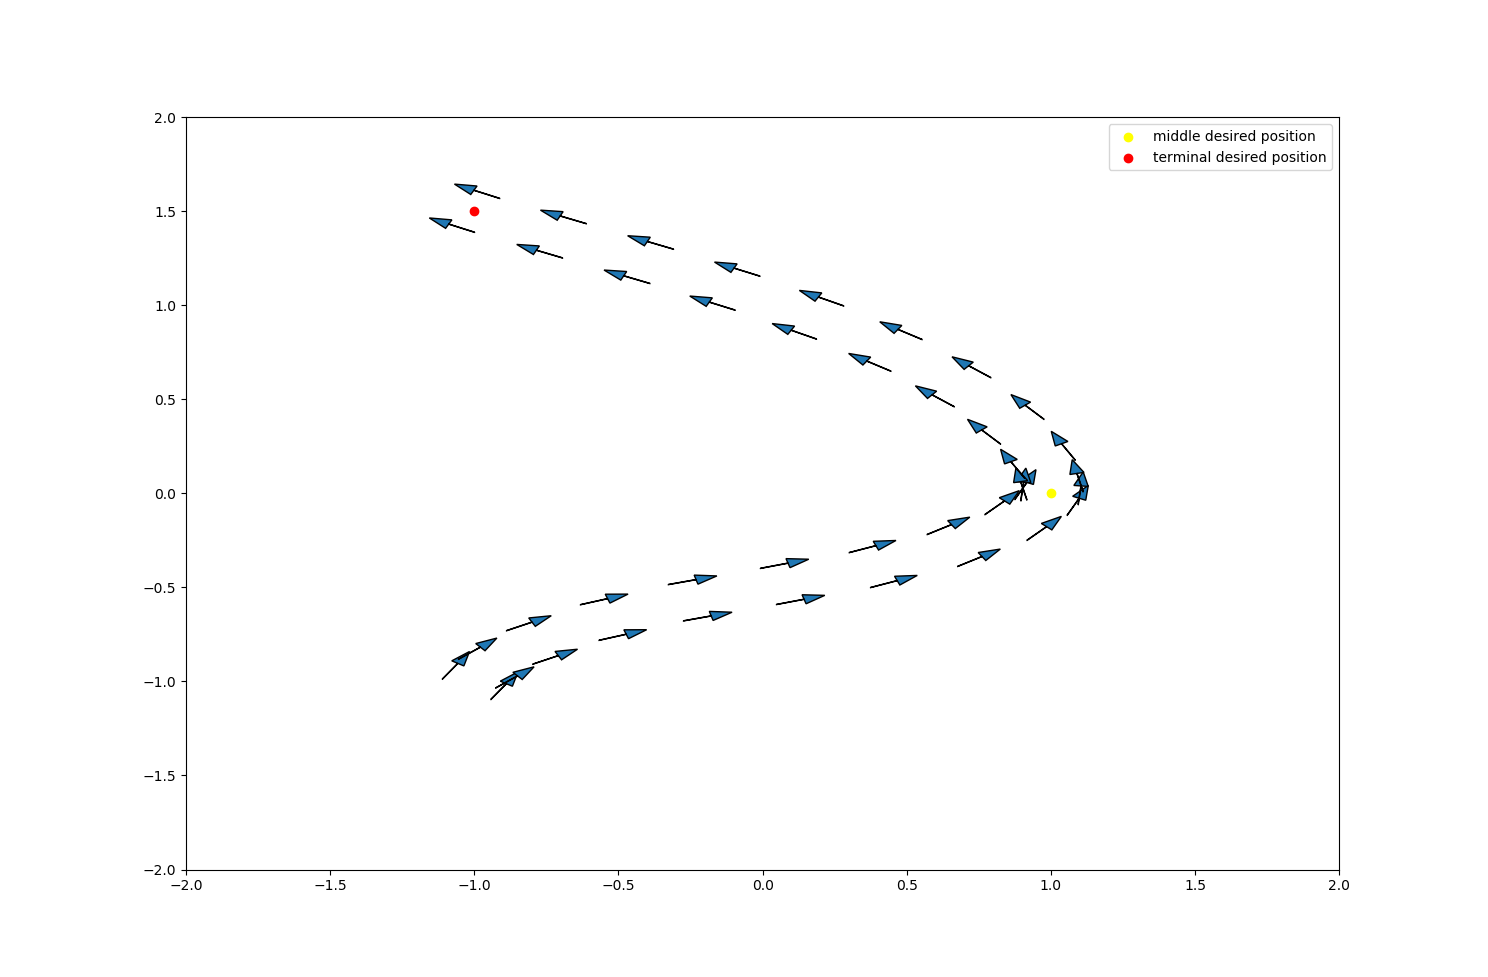
\includegraphics[scale=0.3]{images/Unicycle_car}
\end{figure}

\end{frame}

\begin{frame}{{Graph of convergence}}
\begin{figure}
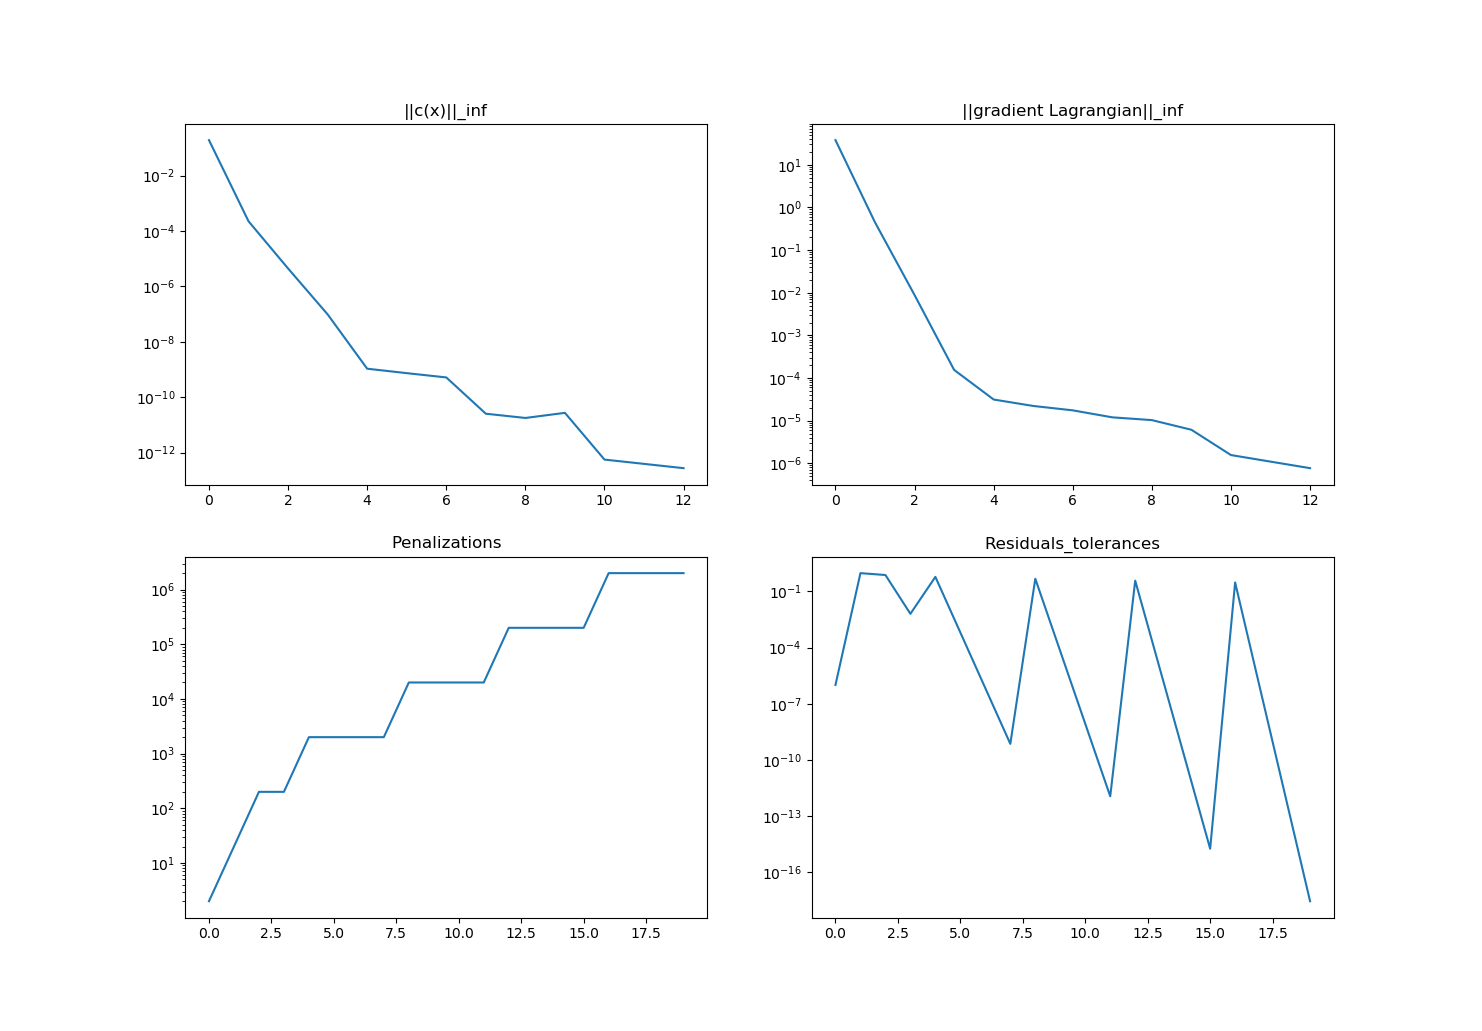
\includegraphics[scale=0.28]{images/Unicycle}
\end{figure}
\end{frame}

\begin{frame}{Difficulty}
\begin{itemize}
\item The theory (of optimization) could be simple
\item The implementation (and debug) could be complex
\item[$\square$] No strong theorem for the convergence of algorithm(s) \footnote{There are indeed many theorems for optimization algorithms, but they are almost always in a weak form or not usable in practice. The special properties they state could be interesting in theory, but they will not directly give convergence guarantee.}
\end{itemize}
\end{frame}

\begin{frame}{Bibliography}
\bibliographystyle{unsrt}
\bibliography{presentation}{}

\end{frame}



\end{document}